\begin{figure}[tb]
  \centering
  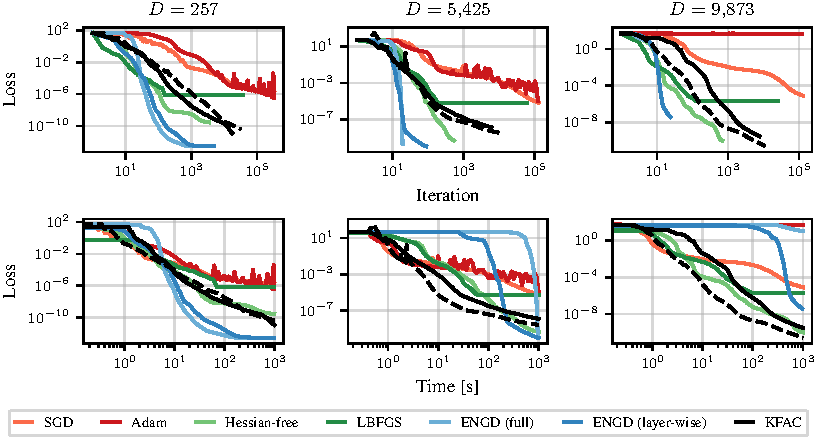
\includegraphics{../kfac_pinns_exp/exp17_groupplot_poisson2d/loss.pdf}
  \caption{Scaling behaviour of different optimizers for learning the solution of a 2d-Poisson equation w.r.t.
    neural network size under a given time budget of $10^3\,\text{s}$ on an RTX 6000 GPU.}
  \label{fig:pedagogical-example}
\end{figure}

\subsection{Setup}
\subsection{Implementation and experimental setup}

\paragraph{Implementation details}
\begin{itemize}
    \item how do we combine the interior and boundary approximations?
    \item damping
    \item exponential moving average
    \item line search
    \item combination of interior and boundary approximations and linear solver: Also, the Kronecker sum's inversion requires solving a generalized eigenvalue problem, for which there is currently no API in PyTorch.
    Hence we need to fall back to SciPy, which costs communication overhead because everything needs to be off-loaded to CPU.
    Alternatively, we could summarize the two Kronecker approximations into a single one at the risk of losing downstream performance.
    \todo{which one do we use?}
    \item \paragraph{Stability and memory considerations}
    Our KFAC implementation requires matrix (eigen-)decompositions and uses dense pre-conditioner matrices.
    This can cause numerical instabilities and large memory consumption.
    Both issues can be addressed by using an inverse-free KFAC update~\citep{lin2023simplifying} and structured Kronecker factors~\citep{lin2023structured}.
    We leave this additions to future work.
    One could also merge the backward pass for each Gramian with that of its loss into a single backward traversal rather than two sequential ones, e.g.\,as done by~\cite{dangel2020backpack}.
    However, then one needs to manually implement the additional backpropagation (through both the normal forward pass, but also through the forward Laplacian pass).
\end{itemize}


%%% Local Variables:
%%% mode: latex
%%% TeX-master: "../main"
%%% End:



\paragraph{Experimental setup}
\begin{itemize}
    \item Tested optimizers: Adam, GD with LS?, Newton's method / (L-)BFGS, Full ENGD, (Block)-Diagonal approximation for ENGD?, KFAC-exp, KFAC-for, KFAC-emp? %, other KFACs: for the l2-GN, empirical Fisher, Quantum KFAC
    \item hyper-parameter search
    %\item try without line search with learning rate schedules
\end{itemize}

\subsection{A high dimensional Poisson equation}

\begin{itemize}
    \item 100D from deep Ritz paper~\citep{yu2018deep}, i.e.,
    \begin{align*}
        -\Delta u(x) & = -200 \quad \text{for } x\in [0,1]^{100} \\
        u(x) & = \lVert x \rVert_2^2 \quad \text{for } x\in \partial[0,1]^{100}
    \end{align*}
    where the solution is given by $u^\star(x) = \lVert x \rVert_2^2$
    \item around $10^5$ to $10^6$ parameters
    \item no ENGD, ENGD matrix-free?, only KFACs, L-BFGS, HF, and first-order methods
\end{itemize}

\subsection{A pedagogical example}

\begin{itemize}
    \item pretty much our current 2D / 5D Poisson example
    \item meant as an illustration of how the approximation of KFAC compares to ENGD and ENGD block-diagonal
    \item plot parameters vs iteration time
\end{itemize}

\subsection{Heat equation}

\begin{itemize}
    \item again 100D
    \item sum of cosinuts with exponential trash in time? I.e.,
    time-space domain $[0,1]\times[0,1]^{100}$ %and
    %\begin{align*}
    %    \partial_t u(t,x)-\Delta_x u(t,x) & = 0 \quad \text{for } x\in [0,1]^{100} \\
    %    u(0,x) & = \sum_{i=1}^{100} \sin(\pi x_i) \quad \text{for }
    %    x\in [0,1]^{100}
    %    \\
    %    u(t,x) & = 0 \quad \text{for } t\in[0,1], x\in\partial[0,1]^{100}
    %\end{align*}
    %\item an alternative would be
    \begin{align*}
        \partial_t u(t,x)-\Delta_x u(t,x) & = 0 \quad \text{for } x\in [0,1]^{100} \\
        u(0,x) & = \sum_{i=1}^{100} \sin(\pi x_i) \quad \text{for }
        x\in [0,1]^{100}
        \\
        u(t,x) & = e^{-\pi^2 t}\sum_{i=1}^{100} \sin(\pi x_i) \quad \text{for } t\in[0,1], x\in\partial[0,1]^{100}
    \end{align*}
    for which the solution should be given by
    \begin{align*}
        u^\star(t,x) = e^{-\pi^2 t} \sum_{i=1}^{100} \sin(\pi x_i)?
    \end{align*}
    %we can also scale in time because $e^{-4\pi^2}\approx e^{-40}$
    \item around $10^5-10^6$ parameters
\end{itemize}

\begin{comment}
    We want to show the following things:
\begin{itemize}
\item We can safely discard the Gramian's off-diagonal blocks without harming
  training performance. This reduces the Gramian's size, but still imposes
  strong constraints on scalability.

\item Our proposed Kronecker approximation works roughly as well as the
  full/block diagonal Gramian, while being much cheaper to compute, store, and
  invert.

\item Thanks to the Kronecker approximation of the Gramian, we can scale to larger neural networks where the other methods either do not work (storing the Gramian is prohibitively expensive) or become quite slow (matrix-free linear system solve via Gramian-vector products).
\end{itemize}

Todos:
\begin{itemize}
\item concrete example ground truth: 2d Poisson on unit square with sine target
\end{itemize}

Ideas:
\begin{itemize}
\item try out different approximations
  \begin{itemize}
  \item Ground truth
  \item Block diagonal exact
  \item Diagonal
  \item Block diagonal with different approximations
  \end{itemize}
\end{itemize}
\end{comment}

%%% Local Variables:
%%% mode: latex
%%% TeX-master: "../main"
%%% End:
